\documentclass[titlepage=true, parskip=full]{scrartcl}
\usepackage[utf8]{inputenc} % use utf8 file encoding for TeX sources
\usepackage[T1]{fontenc}    % avoid garbled Unicode text in pdf
\usepackage{palatino}	      % because "Computer Modern" standard font is illegible
\usepackage{mathpazo}
\usepackage{amsmath}
\usepackage[ngerman]{babel}  % german hyphenation, quotes, etc
\usepackage{hyperref}       % detailed hyperlink/pdf configuration
\hypersetup{                % ‘texdoc hyperref‘ for options
	pdftitle={PSE: Implementierungsbericht},%
	bookmarks=true,%
}
\usepackage{graphicx}       % provides commands for including figures
\usepackage{csquotes}       % provides \enquote{} macro for "quotes"
\usepackage[nonumberlist, numberedsection]{glossaries}     % provides glossary commands
\usepackage{enumitem}
\usepackage{tikz}
%\usepackage{tikz-uml}
%\usepackage{tikz-er2}
\usepackage{comment}
\usepackage{array}
\usepackage{longtable}
\usepackage{hhline}
\usepackage{placeins}
\usepackage{needspace}
\usepackage[toc, page]{appendix}
\usepackage{tabularx}
\usepackage{tabulary}
\usepackage{multirow}
\usepackage{multicol}
\usepackage{rotating}
\usepackage{microtype}
\usepackage{MnSymbol}
\usetikzlibrary{positioning}
\usepackage{pgfgantt}
\usepackage{float}
%\usepackage{listings}
\usepackage{xcolor}

\colorlet{punct}{red!60!black}
\definecolor{background}{HTML}{EEEEEE}
\definecolor{delim}{RGB}{20,105,176}
\colorlet{numb}{magenta!60!black}

% Kommandos für Atomare und JSON-Werte:
\newcommand{\jsonatom}[1]{$\langle\textnormal{\textit{#1}}\rangle$}
\newcommand{\jsonobj}[1]{$\llangle\textnormal{\textit{#1}}\rrangle$}
\newcommand{\jsonpart}[2]{$\llangle\textnormal{\textit{#1}\,[#2]}\rrangle$}

\lstdefinelanguage{json}{
    basicstyle=\normalfont\ttfamily,
    numbers=left,
    numberstyle=\scriptsize,
    escapeinside={(*}{*)},
    stepnumber=1,
    numbersep=8pt,
    showstringspaces=false,
    breaklines=true,
    frame=lines,
    backgroundcolor=\color{background},
    literate=
     *{0}{{{\color{numb}0}}}{1}
      {1}{{{\color{numb}1}}}{1}
      {2}{{{\color{numb}2}}}{1}
      {3}{{{\color{numb}3}}}{1}
      {4}{{{\color{numb}4}}}{1}
      {5}{{{\color{numb}5}}}{1}
      {6}{{{\color{numb}6}}}{1}
      {7}{{{\color{numb}7}}}{1}
      {8}{{{\color{numb}8}}}{1}
      {9}{{{\color{numb}9}}}{1}
      {:}{{{\color{punct}{:}}}}{1}
      {,}{{{\color{punct}{,}}}}{1}
      {\{}{{{\color{delim}{\{}}}}{1}
      {\}}{{{\color{delim}{\}}}}}{1}
      {[}{{{\color{delim}{[}}}}{1}
      {]}{{{\color{delim}{]}}}}{1},
}


%\usepackage[vlined]{algorithm2e}
% see http://ctan.math.utah.edu/ctan/tex-archive/macros/latex/contrib/algorithm2e/doc/algorithm2e.pdf  for more information
\DontPrintSemicolon
\SetKwSwitch{Switch}{Case}{Other}{case}{of}{}{else}{}{}
\SetKw{KwAssert}{assert}
\SetKw{KwInvariant}{invariant}
\SetKw{KwStep}{step}
\SetKw{KwDownto}{downto}	
\SetKw{KwArrayOf}{array of }
\SetKw{KwArray}{array }
\SetKw{KwOf}{ of }
\SetKw{KwNot}{ not }
\SetKw{KwIs}{ is }
\SetKw{KwAnd}{ and }
\SetKw{KwOr}{ or }
\SetKw{KwBreak}{break}
\SetKw{KwThrow}{throw}
\SetKw{KwTrue}{true}
\SetKw{KwFalse}{false}
\SetKwBlock{KwFunc}{function}{}
\SetKwBlock{KwProc}{procedure}{}
\newcommand{\Function}[2]{\KwFunc({#1}){#2}}
\newcommand{\Procedure}[2]{\KwProc({#1}){#2}}
\SetKwData{KwList}{List}
\SetKwData{KwSet}{Set}
\newcommand{\KwListOf}{\KwList \KwOf}
\newcommand{\KwSetOf}{\KwSet \KwOf}
\SetKwComment{Comment}{// }{}
\newcommand{\LComment}[1]{\hspace{-2pt}\Comment*[l]{#1}}
\newcommand{\RComment}[1]{$ \qquad $ \Comment*[h]{#1} \\}
\newcommand{\RCommentNoBreak}[1]{$ \qquad $ \Comment*[h]{#1}}
\newcommand{\MyCommentSty}[1]{\emph{\textcolor{gray}{#1}}}
\SetCommentSty{MyCommentSty}
\SetFuncSty{emph}
\definecolor{kwblue}{rgb}{0.3,0.3,1}
\newcommand{\MyKwSty}[1]{\textcolor{kwblue}{\textbf{#1}}}
\SetKwSty{MyKwSty}
\newcommand{\Call}[2]{\FuncSty{#1}(#2)}
\newcommand{\pluseq}{\mathrel{+}=}
\newcommand{\Var}[1]{\textit{#1}}

% needed to define linebreak points without hyphenation (useful for URL wrapping)
\newcommand{\+}{\discretionary{}{}{}}

\renewcommand{\arraystretch}{1.24}  % for proper row spacing in tables

%%%%%%%%%%%%%%%%%%%%%%%%%%%
% longtable multirow page break insanity fix – http://tex.stackexchange.com/a/52101
\makeatletter
\def\@cline#1-#2\@nil{%
	\omit
	\@multicnt#1%
	\advance\@multispan\m@ne
	\ifnum\@multicnt=\@ne\@firstofone{&\omit}\fi
	\@multicnt#2%
	\advance\@multicnt-#1%
	\advance\@multispan\@ne
	\leaders\hrule\@height\arrayrulewidth\hfill
	\cr
	\noalign{\nobreak\vskip-\arrayrulewidth}}
\makeatother
%%%%%%%%%%%%%%%%%%%%%%%%%%%

% For Christ's sake, I'm sick and tired of this f*cking orphan/widow crap!
\widowpenalty=10000
\clubpenalty=10000
% Source: somewhere on tex.stackexchange.com

\renewcommand{\to}{\longrightarrow} % proper math typography
\newcommand{\NN}{\mathbb{N}}
\newcommand{\RR}{\mathbb{R}}
\newcommand{\QQ}{\mathbb{Q}}

\addto\captionsngerman{\let\appendixtocname\appendixname\let\appendixpagename\appendixname}

% fix hyphenation
\hyphenation{Log-out Log-in Ak-tions Ak-tion ge-öff-net liken dis-liken Like Dis-like No-ti-fi-ca-tion Mo-dule inkl Au-tho-ri-za-tion Web-App Ar-chi-tek-tur-en Ge-ne-rie-rungs Stu-di-en-plan Client}

\usepackage{enumitem}
\setlist[itemize]{nosep}
\shorthandon{"}
%\makeglossaries
%%
% % Automatisch generiertes Glossar
%
%\glsaddall % das sorgt dafür, dass alles Glossareinträge gedruckt werden, nicht nur die verwendeten. Das sollte nicht nötig sein!
%
% % Glossareinträge
%
\newglossaryentry{Rest}
{
	name=REST,
	description={Abk. für Representational State Transfer, Programmierparadigma für \glspl{Webservice} auf Basis des HTTP-Protokolls}
}

\newglossaryentry{ECTS-Punkte}
{
	name=ECTS-Punkte,
	description={Leistungspunkte, die für ein erfolgreich absolviertes \gls{Modul} von der Hochschule auf Basis des ECTS-Punktesystems vergibt werden, und mit denen der Arbeitsaufwand gemessen wird},
}

\newglossaryentry{Generierungs-Tool}
{
	name=Generierungs-Tool,
	description={Tool, für die automatische Erstellung bzw. Vervollständigung von Studienpläne},
}


\newglossaryentry{Webservice}
{
	name=Webservice,
	plural=Webservices,
	description={Softwareanwendung, die über ein Netzwerk bereitgestellt wird}
}

\newglossaryentry{Plug-In-Paket}
{
	name=Plug-In-Paket,
	plural=Plug-In-Pakete,
	description={Paket bestehend aus mehreren \glspl{Plug-In}}
}

\newglossaryentry{iMage}
{
	name={iMage},
	description={Bildbearbeitungssoftware der Firma SWT. Bietet im Basispaket nur Funktionalitäten zur Skalierung und Drehung von Bildern}
}

\newglossaryentry{Internetbrowser}
{
	name={Internetbrowser},
	description={Programm, mit dem Websites gefunden, gelesen und verwaltet werden können, mit aktiviertem JavaScript}
}

\newglossaryentry{Online-Shop}
{
	name={Online-Shop},
	description={Internetseite, die Produkte zum Kauf anbietet}
}

\newglossaryentry{KIT}
{
	name=KIT,
	description={Das Karlsruher Institut für Technologie ist die Forschungsuniversität in der Helmholtz-Gemeinschaft. Standort der Universität ist Karlsruhe. }
}

\newglossaryentry{SCC}
{
	name=SCC,
	plural=SCC,
	description={Das Steinbuch Center for Computing ist ein Institut und das zentrale Rechenzentrum des \gls{KIT}s.}
}

\newglossaryentry{Benutzer}
{
	name=Benutzer,
	plural=Benutzer,
	description={Ein am \gls{KIT} eingeschriebener Student, der über ein gültigen Account beim \gls{SCC} verfügt.}
}

\newglossaryentry{Wizard}
{
	name=Wizard,
	plural=Wizards,
	description={Ein Wizard ist ein Subsystem, welches einen \gls{Benutzer} visuell durch eine Systemfunktionalität führt und dabei vom \gls{Benutzer} bestimmte Interaktionen mit dem System fordert.}
}

\newglossaryentry{Drag-and-Drop}
{
	name=Drag-and-Drop,
	description={(deutsch: "Ziehen und Ablegen") Eine Methode zur Bedienung grafischer Benutzeroberflächen bei der grafische Elemente mittels eines Mauszeigers bewegt werden.}
}

\newglossaryentry{Shibboleth Identity Provider}
{
	name=Shibboleth Identity Provider,
	description={Ein genau spezifiziertes System zum Login mittels einer von einer dritten Instanz bereitgestellten Identität.}
}

\newglossaryentry{Studiengang}
{
	name=Studiengang,
	description={Ein vom KIT angebotener, auf einer Studien- und Prüfungsordnung und einem Modulhandbuch basierender Studiengang.}
}

\newglossaryentry{Semester des Studienbeginns}
{
	name=Semester des Studienbeginns,
	description={Das Semester in welchem der \gls{Benutzer} im ersten Fachsemester des \gls{Studiengang}s war.}
}

\newglossaryentry{Modul}
{
	name=Modul,
	plural=Module,
	description={Ein Modul ist ein Teilblock des Studiums, welcher aus verschiedenartigen Veranstaltungen (genannt \glspl{Teilmodul}) bestehen kann und für welchen man nach Ablegung eventueller \glspl{Modulpruefung} eine festgelegte Anzahl an ECTS-Punkten erhält.}
}
\newglossaryentry{Teilmodul}
{
	name=Teilmodul,
	plural=Teilmodule,
	description={Ein Teilmodul ist eine universitäre Veranstaltung, welche als Teil eines Moduls besucht werden kann und mittels einer (wie auch immer gearteten) \gls{Modulpruefung} bestanden werden kann.}
}
\newglossaryentry{Modulpruefung}
{
	name=Modulprüfung,
	plural=Modulprüfungen,
	description={Eine Modulprüfung ist eine Prüfung, welche abgelegt werden muss um ein Modul \glslink{Modul abgeschlossen}{abzuschließen}.}
}
\newglossaryentry{Zur Pruefung angetreten}
{
	name=Zur Pruefung angetreten,
	description={Ein \gls{Benutzer} ist zu einer \gls{Modulpruefung} angetreten, wenn er sich fristgerecht für selbige angemeldet und nicht fristgerecht abgemeldet hat.}
}

\newglossaryentry{Modul abgeschlossen}
{
	name=Modul abgeschlossen,
	description={Ein \gls{Modul} gilt als abgeschlossen, wenn der \gls{Benutzer} alle nach Modulhandbuch notwendigen \glspl{Modulpruefung} bestanden hat.}
}

\newglossaryentry{Modul begonnen}
{
	name=Modul begonnen,
	description={Ein \gls{Modul} gilt als begonnen, wenn der \gls{Benutzer} zu mindestens einer \gls{Modulpruefung} \glslink{Zur Pruefung angetreten}{angetreten} ist.}
}

\newglossaryentry{Studienplan}
{
	name=Studienplan,
	plural=Studienpläne,
	description={Eine Zusammenstellung von Modulen, in welcher enthalten ist wann welches Modul planmäßig \glslink{Modul begonnen}{begonnen} werden soll.}
}
\shorthandoff{"}

\begin{document}
	
\begin{titlepage}
	\centering
	{\huge \bfseries \sffamily Studienplanung als Generierung von Workflows mit Compliance-Anforderungen: Planerstellung und Visualisierung\par}
	\vspace{1cm}
	{\LARGE Testbericht\par}
	\vfill
	\begin{tabular}{>{\Large}c}
		Nada Chatti\\
		\textbf{Daniel Jungkind}\\
		Hannes Kuchelmeister\\
		Ulrike Rheinheimer\\
		Paul Samuel M. Teuber\\
		Tim Niklas Uhl
	\end{tabular}
	\vfill
	15. März 2017
\end{titlepage}
\tableofcontents
\pagebreak

%
% % Hier beginnt die Gliederung des Pflichtenhefts
\section{Einleitung}
Der Implementierungsbericht des Projekts „Studienplanung als Generierung von Workflows mit Compliance-Anforderungen: Planerstellung und Visualisierung“ beschreibt die Umsetzung des zuvor im Pflichtenheft und Entwurf spezifizierten Projekts. In über ????? Zeilen Java-, Javascript-, HTML- und CSS-Code liegt jetzt eine fertige, nur noch zu optimierende Anwendung vor. In diesem Bericht möchten wir dabei auf implementierte und ausgelassen Features eingehen, Änderungen beschreiben und begründen, und die Implementierungsphase (einschließlich aller durchgemachten Nächte) reflektieren.
Zusammenfassend ist dieser Bericht Ende einer arbeitsintensiven, aber erfolreichen Phase, die als Endprojekt ein einmalig sinnvolles, dringendnotweniges und jedem Studenten zu empfehlendes Studienplanungshilfsmittel zur Verfügung stellt.






\newpage
\begin{appendices}
	\newpage
\FloatBarrier
\section{Bilder}
\begin{figure}[!h]
	\caption{Systemmodell}
	\label{system_model:overview}
	\resizebox{\textwidth}{!} {
		\section{Systemmodelle}
\begin{figure}[!htb]
	\resizebox{\textwidth}{!} {
		\section{Systemmodelle}
\begin{figure}[!htb]
	\resizebox{\textwidth}{!} {
		\input{diagrams/system_model}
	}
\end{figure}
Das System basiert auf einer Client-Server-Architektur mit einer starken Trennung zwischen der Benutzerschnittstelle und dem Anwendungsserver. Der Nutzer gibt die benötigten Daten über die Benutzerschnittstelle ein. Die Verarbeitung findet serverseitig statt. Die \gls{Weboberflaeche} sendet hierfür eine Anfrage über einen \gls{Rest}-\gls{Webservice}
 und erhält über diese Schnittstelle eine Antwort zurück. \\
Auf dem Anwendungsserver werden die notwendigen Berechnungen durchgeführt, sowie die Produktdaten verarbeitet und gesichert.
	}
\end{figure}
Das System basiert auf einer Client-Server-Architektur mit einer starken Trennung zwischen der Benutzerschnittstelle und dem Anwendungsserver. Der Nutzer gibt die benötigten Daten über die Benutzerschnittstelle ein. Die Verarbeitung findet serverseitig statt. Die \gls{Weboberflaeche} sendet hierfür eine Anfrage über einen \gls{Rest}-\gls{Webservice}
 und erhält über diese Schnittstelle eine Antwort zurück. \\
Auf dem Anwendungsserver werden die notwendigen Berechnungen durchgeführt, sowie die Produktdaten verarbeitet und gesichert.
	}
\end{figure}
\begin{figure}[!h]
	\caption{Loginseite des Systems mit Anmeldung über den \gls{Shibboleth Identity Provider} des \gls{KIT}}
	\label{fig:gui-login-1}
	\centering
	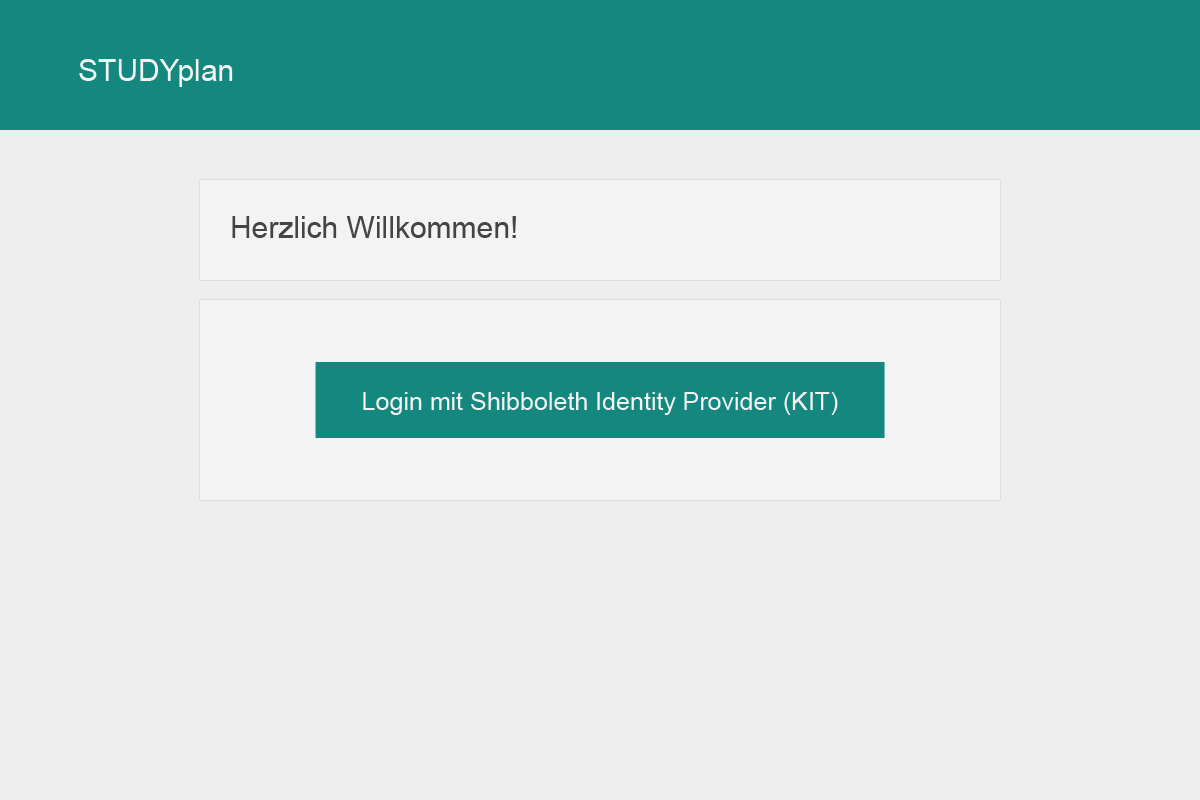
\includegraphics[width=0.8\textwidth]{../GUI/ergebnisse/login-1.png}
\end{figure}
\begin{figure}[!h]
	\caption{Erste Seite des Registrierungs"=\gls{Wizard}s mit Eingabe von Studienfach und Studienbeginn}
	\label{fig:gui-registrierung-1}
	\centering
	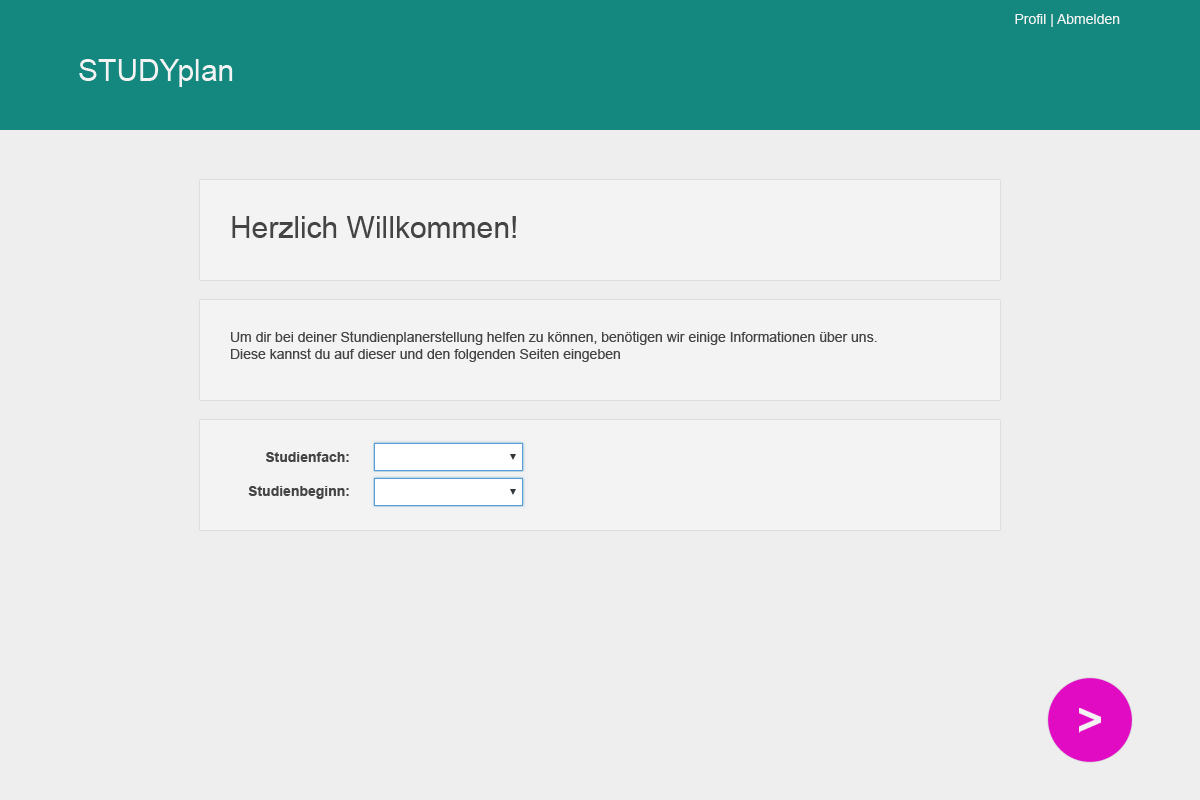
\includegraphics[width=0.8\textwidth]{../GUI/ergebnisse/registrierung-1.png}
\end{figure}

\begin{figure}
	\caption{Zweite Seite des Registrierungs"=\gls{Wizard}s mit Eingabe der schon begonnenen Module}
	\label{fig:gui-registrierung-2}
	\centering
	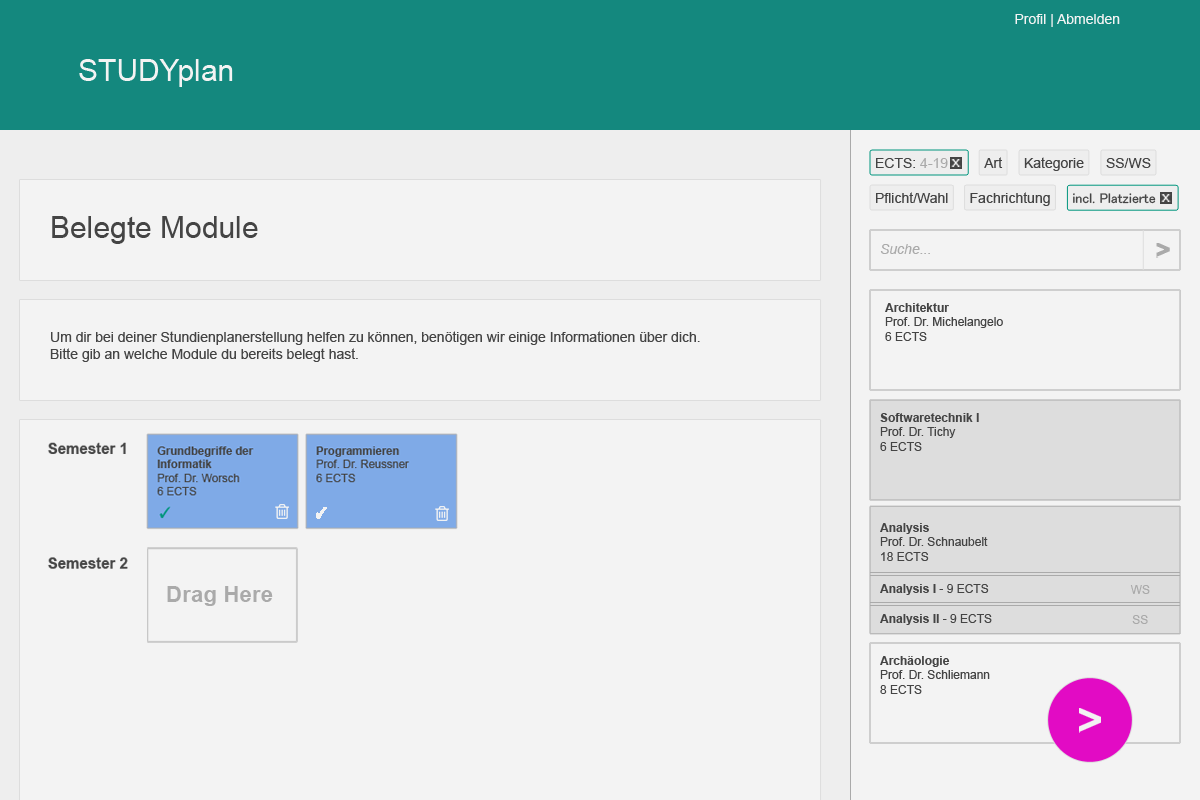
\includegraphics[width=0.9\textwidth]{../GUI/ergebnisse/registrierung-2.png}
\end{figure}

\begin{figure}
	\caption{Hauptseite des Systems}
	\label{fig:gui-hauptseite-1}
	\centering
	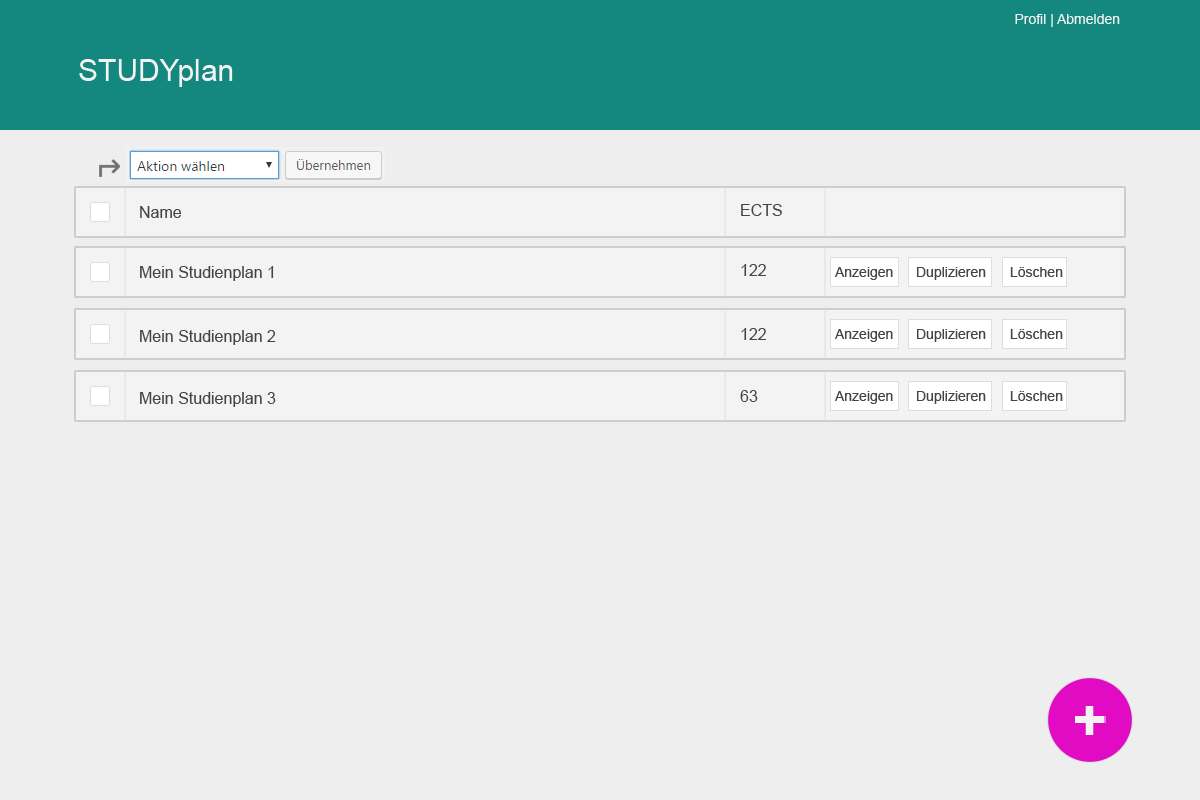
\includegraphics[width=0.9\textwidth]{../GUI/ergebnisse/hauptseite-1.png}
\end{figure}
\begin{figure}
	\caption{Manuelle Bearbeitung des Studienplans}
	\label{fig:gui-bearbeitung-1}
	\centering
	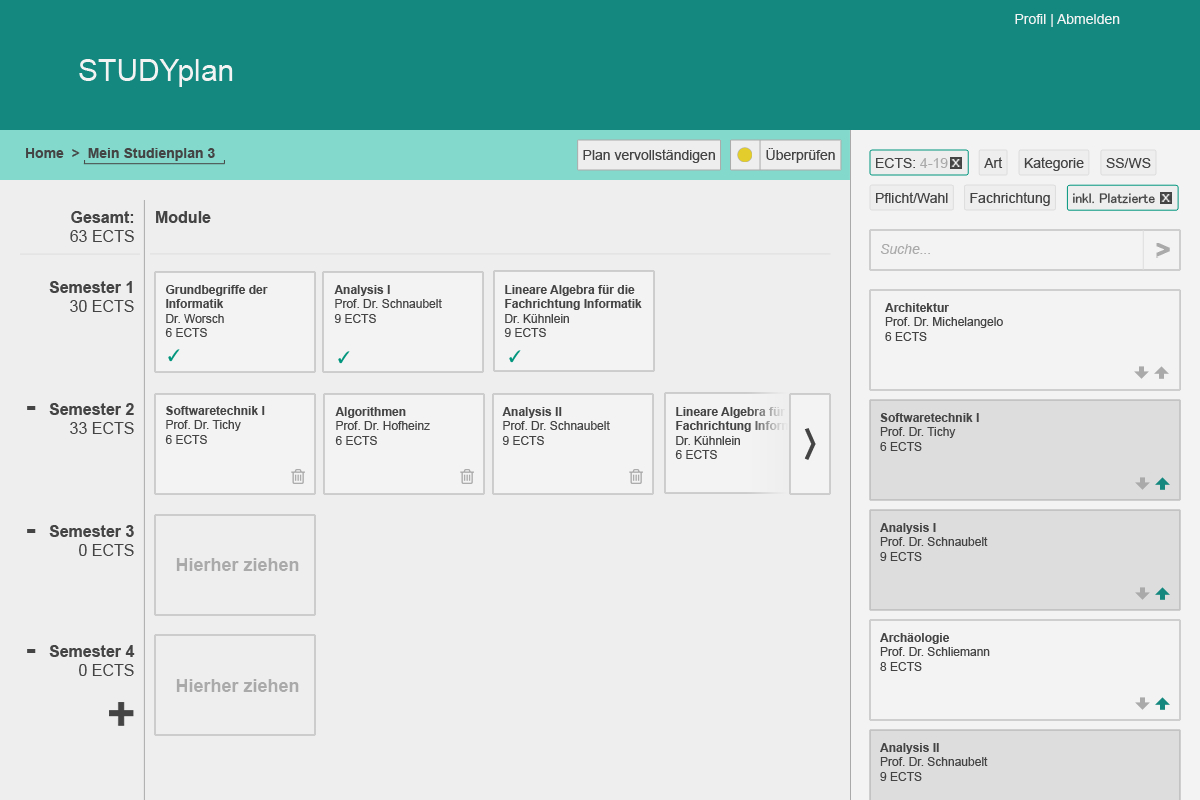
\includegraphics[width=0.9\textwidth]{../GUI/ergebnisse/bearbeitung-1.png}
\end{figure}
\begin{figure}
	\caption{Seitenleiste für Modulfilterung mit offener Kategorie-Auswahl}
	\label{fig:gui-module-filtern-1}
	\centering
	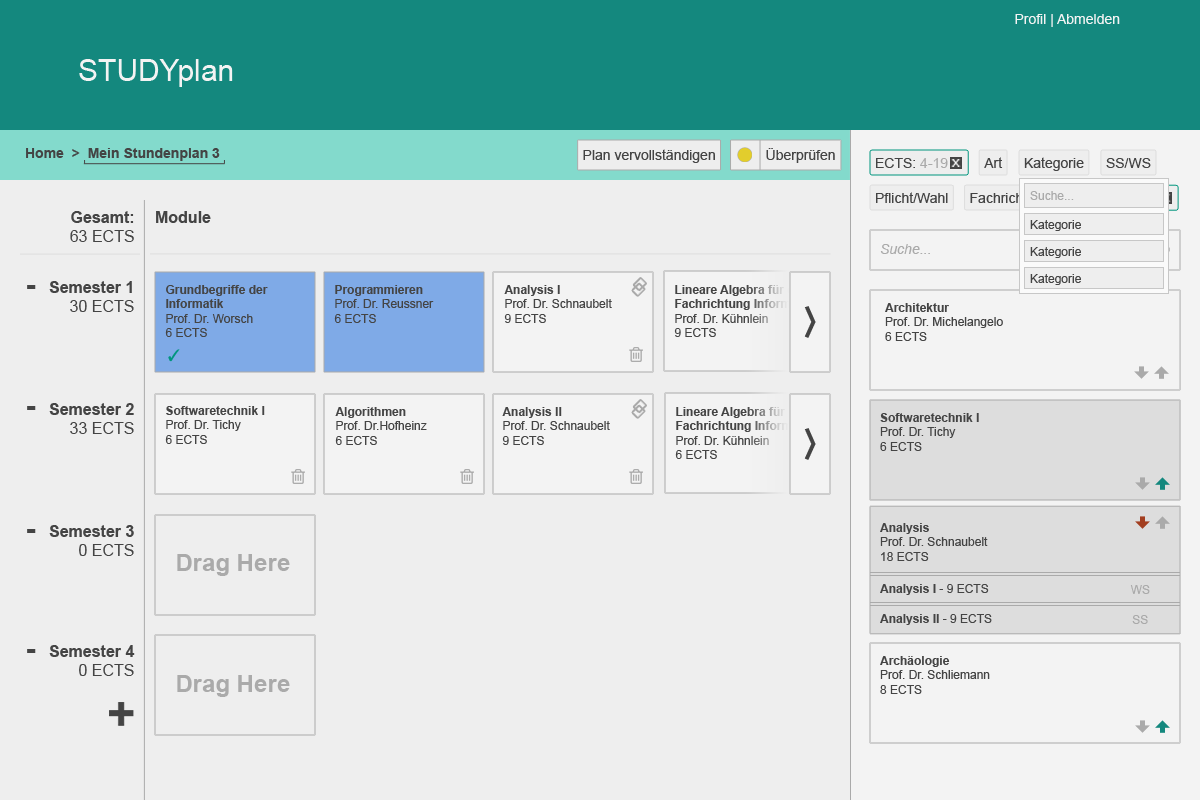
\includegraphics[width=0.9\textwidth]{../GUI/ergebnisse/module-filtern-1.png}
\end{figure}
\begin{figure}
	\caption{Seitenleiste für Modulfilterung mit offener ECTS-Auswahl}
	\label{fig:gui-module-filtern-2}
	\centering
	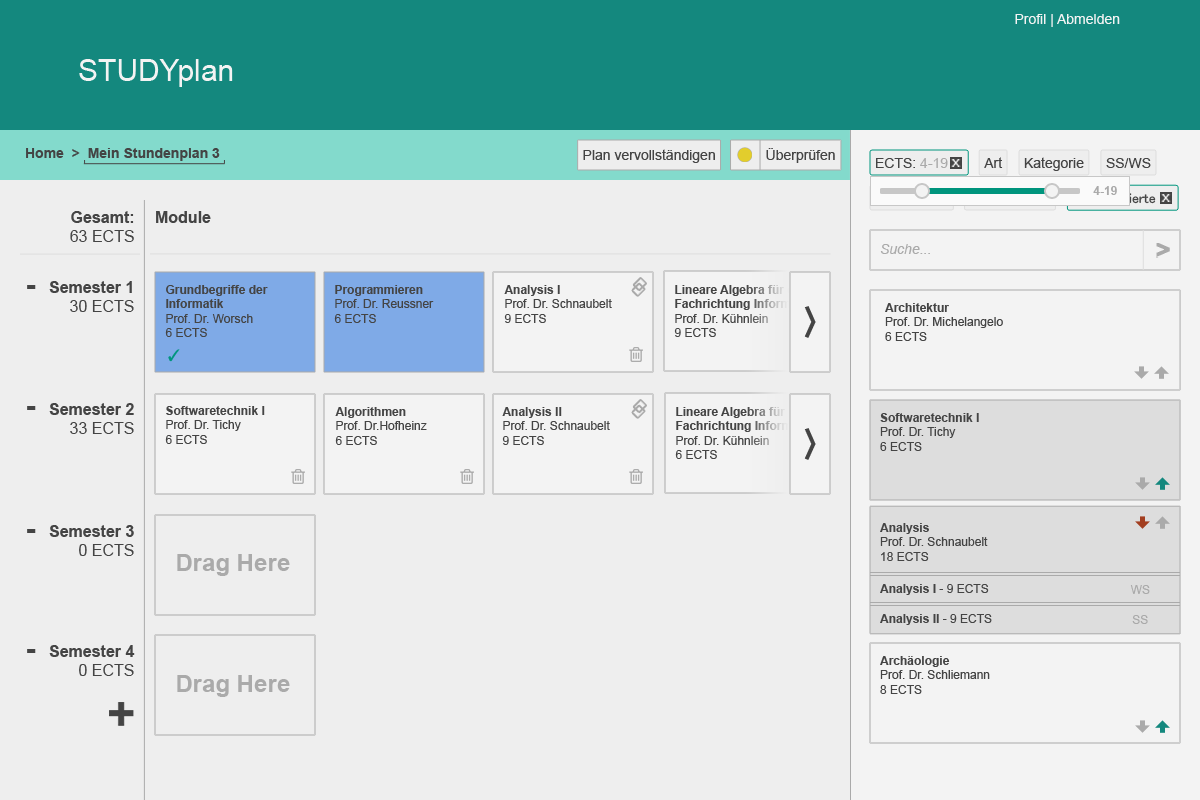
\includegraphics[width=0.9\textwidth]{../GUI/ergebnisse/module-filtern-2.png}
\end{figure}
\begin{figure}
	\caption{Detailansicht für Modul}
	\label{fig:gui-modul-info-1}
	\centering
	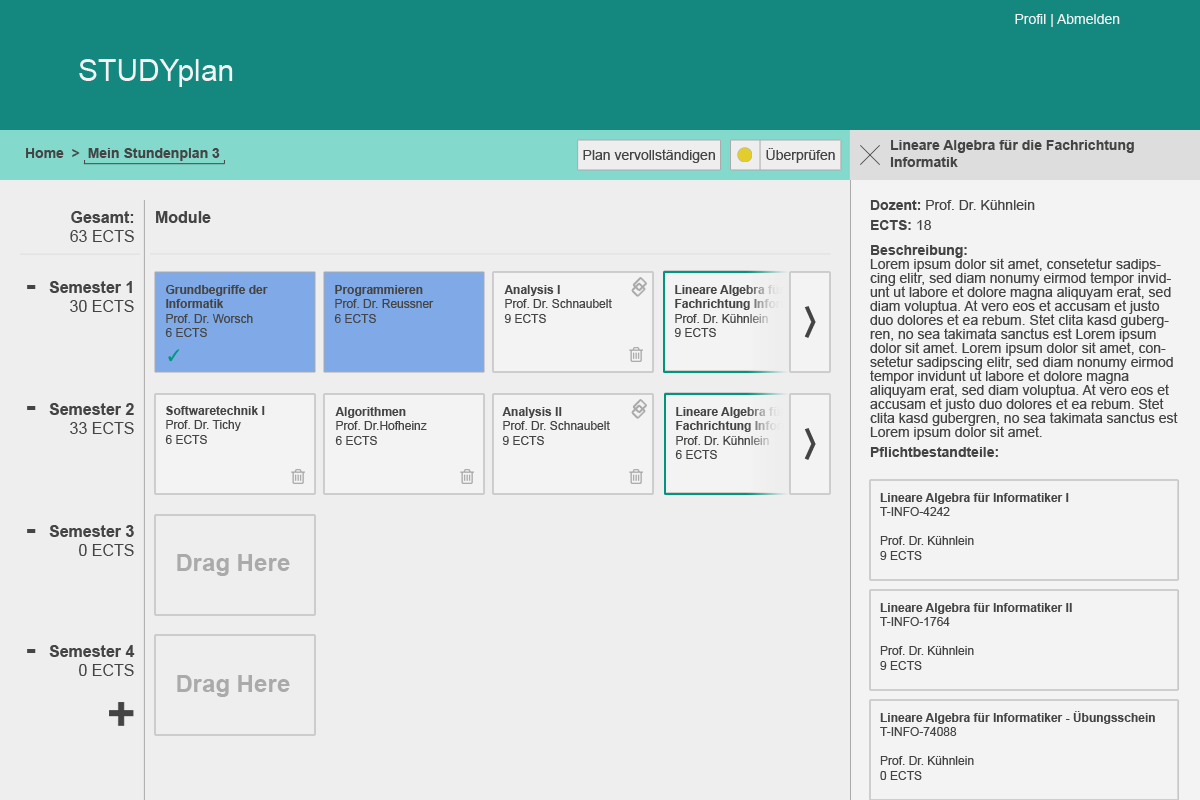
\includegraphics[width=0.9\textwidth]{../GUI/ergebnisse/modul-info-1.png}
\end{figure}
\begin{figure}
	\caption{1. Seite des Generierungs-Wizards}
	\label{fig:gui-generierung-1}
	\centering
	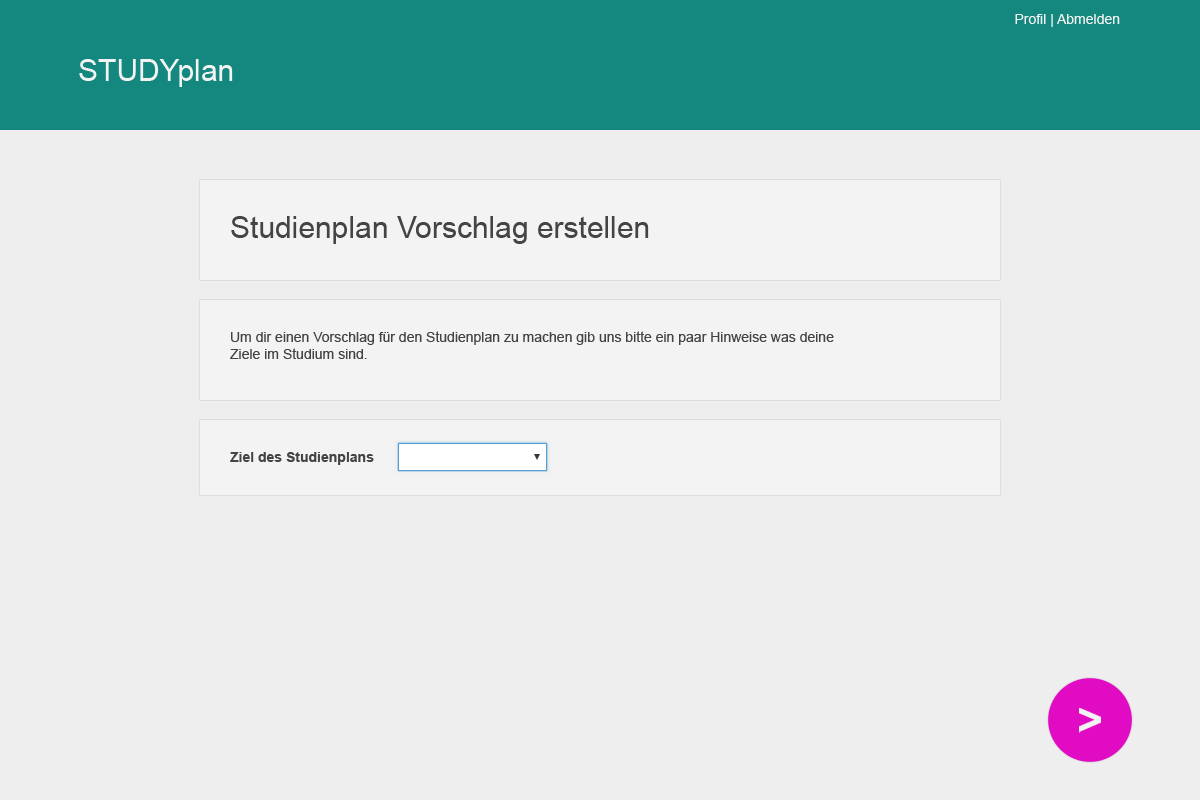
\includegraphics[width=0.9\textwidth]{../GUI/ergebnisse/generierung-1.png}
\end{figure}

\begin{figure}
	\caption{2. Seite des Generierungs-Wizard}
	\label{fig:gui-generierung-2}
	\centering
	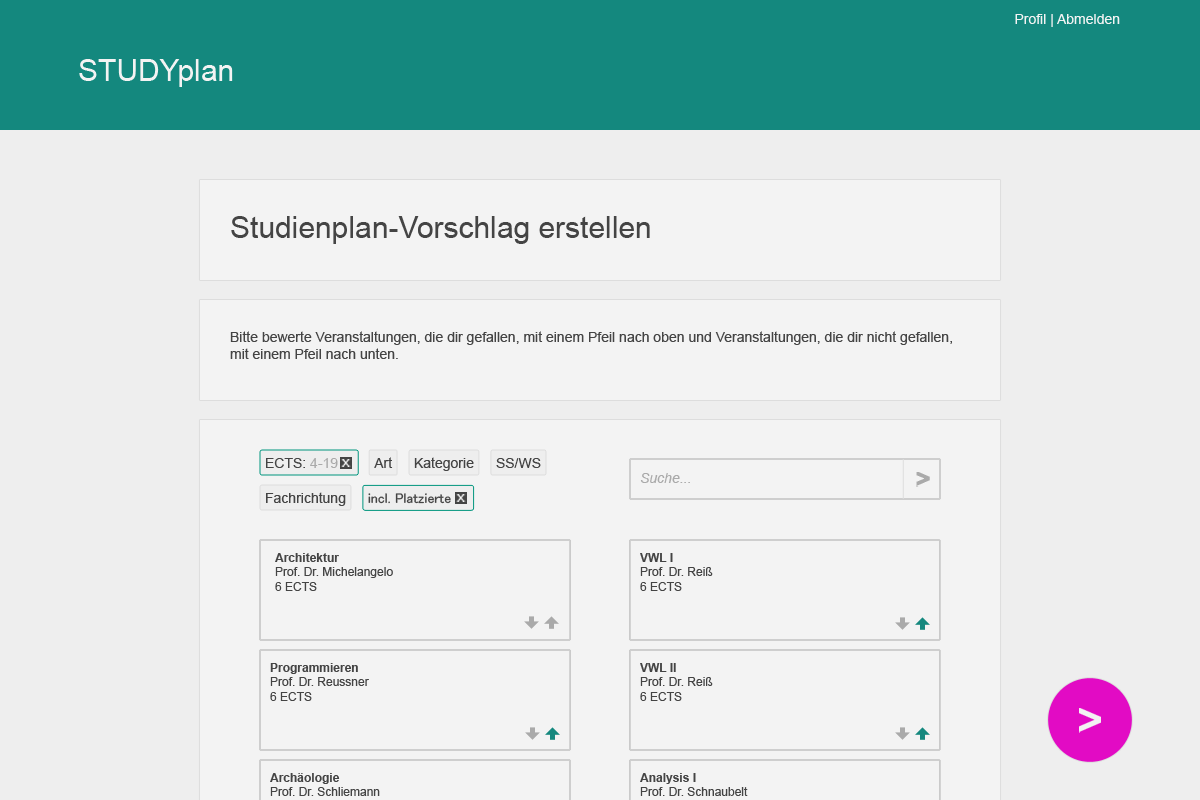
\includegraphics[width=0.9\textwidth]{../GUI/ergebnisse/generierung-2.png}
\end{figure}

\begin{figure}
	\caption{3. Seite des Generierungs-Wizard}
	\label{fig:gui-generierung-3}
	\centering
	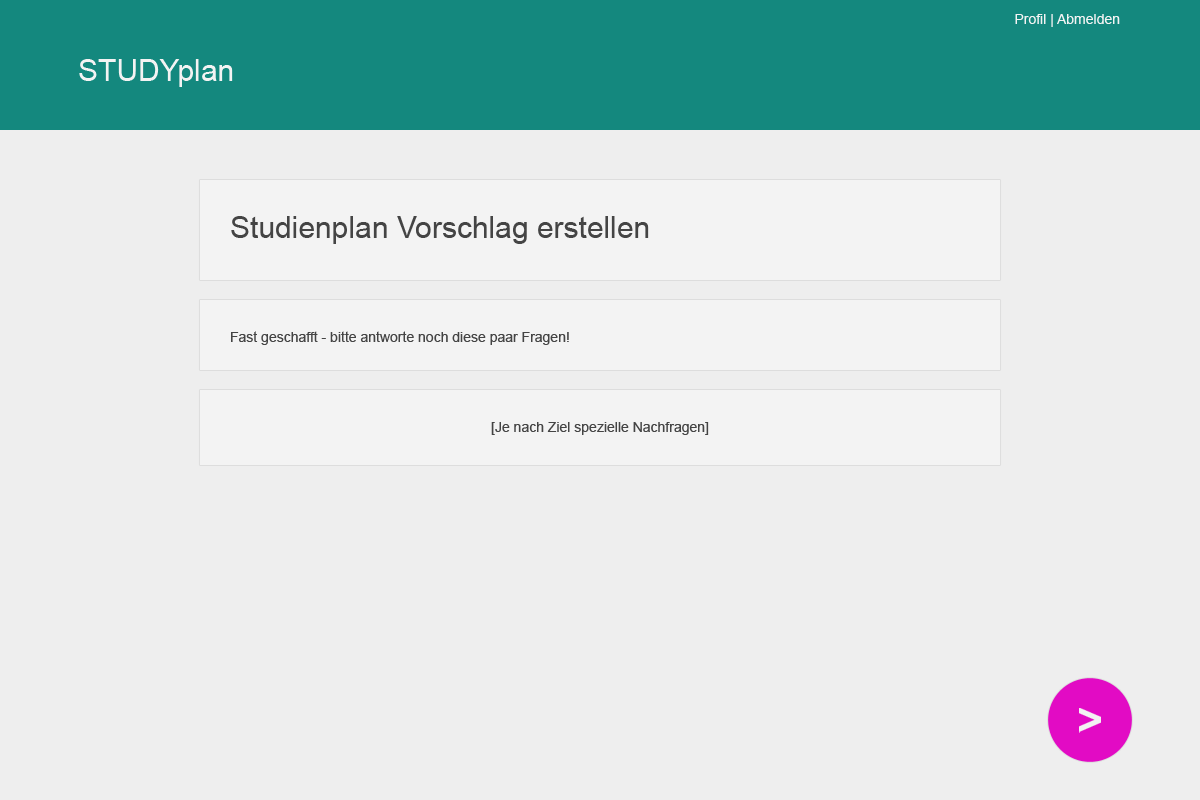
\includegraphics[width=0.9\textwidth]{../GUI/ergebnisse/generierung-3.png}
\end{figure}

\begin{figure}
	\caption{Anzeige des generierten Studienplans}
	\label{fig:gui-generierung-4}
	\centering
	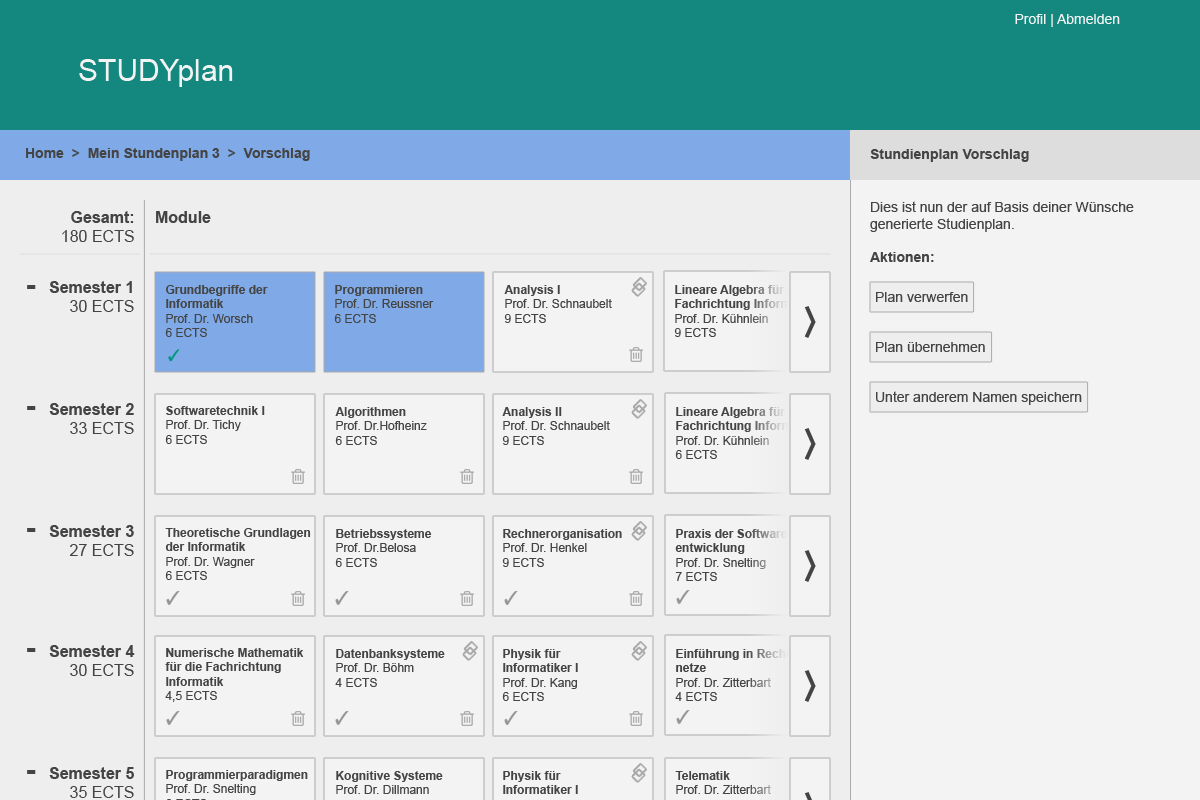
\includegraphics[width=0.9\textwidth]{../GUI/ergebnisse/generierung-4.png}
\end{figure}
\begin{figure}
	\caption{Erfolgreiche Verifizierung}
	\label{fig:gui-verifizierung-1}
	\centering
	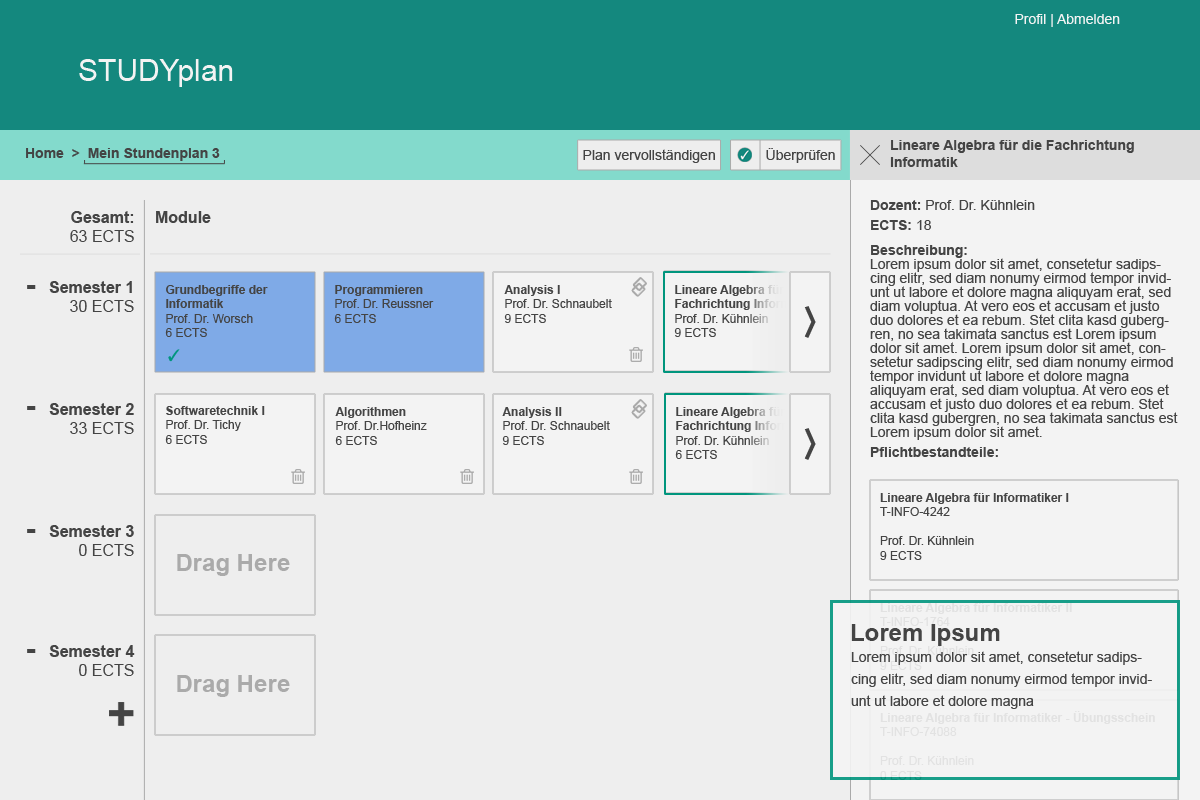
\includegraphics[width=0.9\textwidth]{../GUI/ergebnisse/verifizierung-1.png}
\end{figure}
\begin{figure}
	\caption{Fehlgeschlagene Verifizierung}
	\label{fig:gui-verifizierung-2}
	\centering
	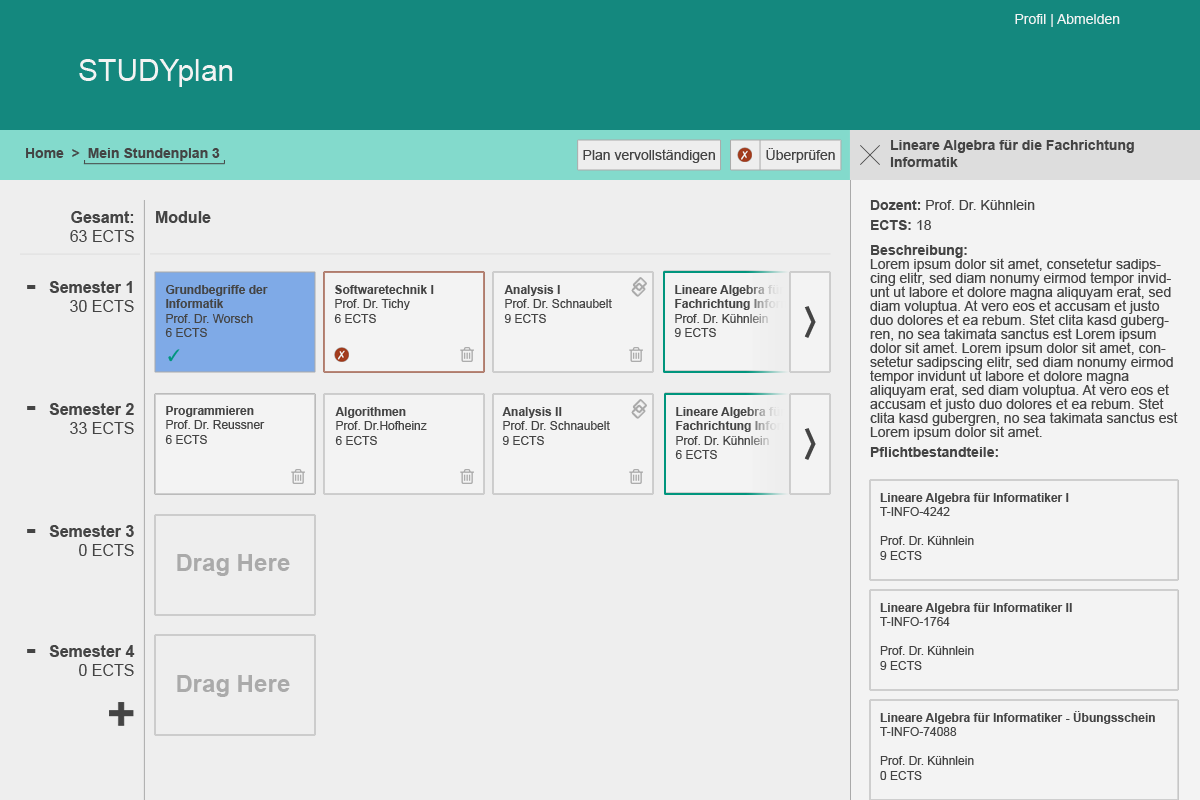
\includegraphics[width=0.9\textwidth]{../GUI/ergebnisse/verifizierung-2.png}
\end{figure}
\begin{figure}
	\caption{Profilansicht}
	\label{fig:gui-profil-1}
	\centering
	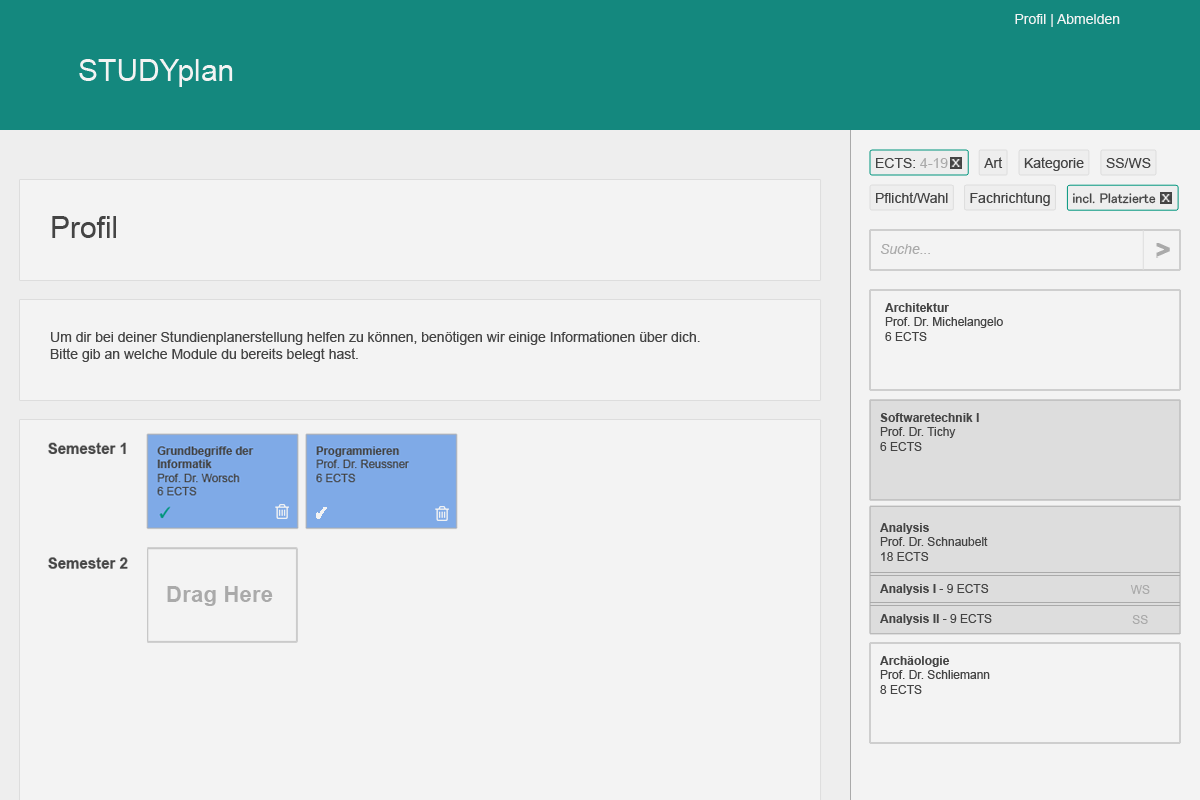
\includegraphics[width=0.9\textwidth]{../GUI/ergebnisse/profil-1.png}
\end{figure}
\FloatBarrier	
\end{appendices}
\end{document}
